\section{Architektúra testovacieho stojanu} \label{s: architektura}

Pre účely výskumu bol navrhnutý a implementovaný izolovaný testovací stojan v prostredí Docker Compose. Stojan pozostáva z dvoch hlavných mikroservisov napísaných v jazyku Go:

\begin{itemize}
\item \textbf{Service A (Generátor záťaže):} Simuluje klientske požiadavky a generuje kontinuálny tok transakcií.
\item \textbf{Service B (Spracovateľ):} Prijíma požiadavky, vykonáva ľahkú biznis logiku a simuluje zápis do databázy.
\end{itemize}

Injekcia sieťových chýb je realizovaná na úrovni kontajnerov pomocou princípov Chaos Engineeringu~\cite{Rosenthal2020, Basiri2016}. Tento prístup umožňuje dynamicky simulovať:
\begin{enumerate}
\item Umelé zvýšenie latencie (Network Latency Jump).
\item Náhodnú stratu paketov (Packet Loss).
\item Kompletné prerušenie sieťového spojenia (Network Partitioning / Split-Brain).
\end{enumerate}

\begin{figure}[htbp]
\centering
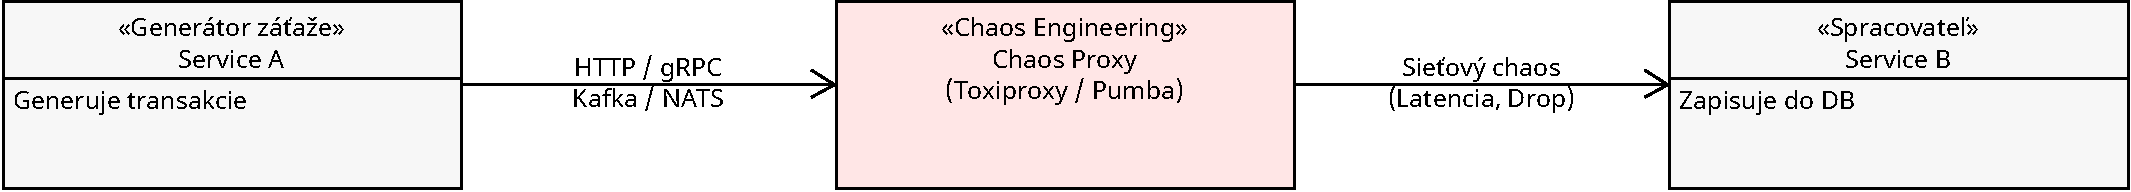
\includegraphics[width=0.8\textwidth]{architektura-crop.pdf}
\caption{Architektúra testovacieho stojanu a injekcia sieťových chýb.}
\label{f:architektura}
\end{figure}

Ako môžeme vidieť na obrázku~\ref{f:architektura}, všetka komunikácia medzi generátorom a spracovateľom prebieha cez prostredníka, ktorý simuluje sieťovú degradáciu.